\begin{frame}
\frametitle{One-dimensional case - Setup}
Consider $D=[-1,1]$ and the SDE
\begin{equation*}
\left \{
\begin{aligned}
	dX(t) &= f(X(t)) dt + g(X(t))dW(t), && 0 < t \leq T, \\
	X(0)  &= X_0, && X_0 \in D.
\end{aligned} \right .
\end{equation*}
Set mixed boundary conditions and
\begin{equation*}
\begin{split}
	f(x) &= -V'(x), \text{ where } V(x) = 0.1(8x^4 - 8x^2 + x + 2), \\
	g(x) &= \sigma \in \R.
\end{split}
\end{equation*}
\underline{Goal}. Verify the weak order of convergence of DEM and CEM.
\underline{Reference solution}. Solution of PDE's
\begin{itemize}
	\item Analytic solution in one-dimensional case for $\bar \tau$,
	\item Finite Differences for $\Phi$.
\end{itemize}
\end{frame}

\begin{frame}
\frametitle{One-dimensional case - Results}
\begin{figure}[t]
    \centering
    \begin{subfigure}{0.49\linewidth}
        \centering
        \resizebox{1\linewidth}{!}{% This file was created by matlab2tikz.
%
%The latest updates can be retrieved from
%  http://www.mathworks.com/matlabcentral/fileexchange/22022-matlab2tikz-matlab2tikz
%where you can also make suggestions and rate matlab2tikz.
%
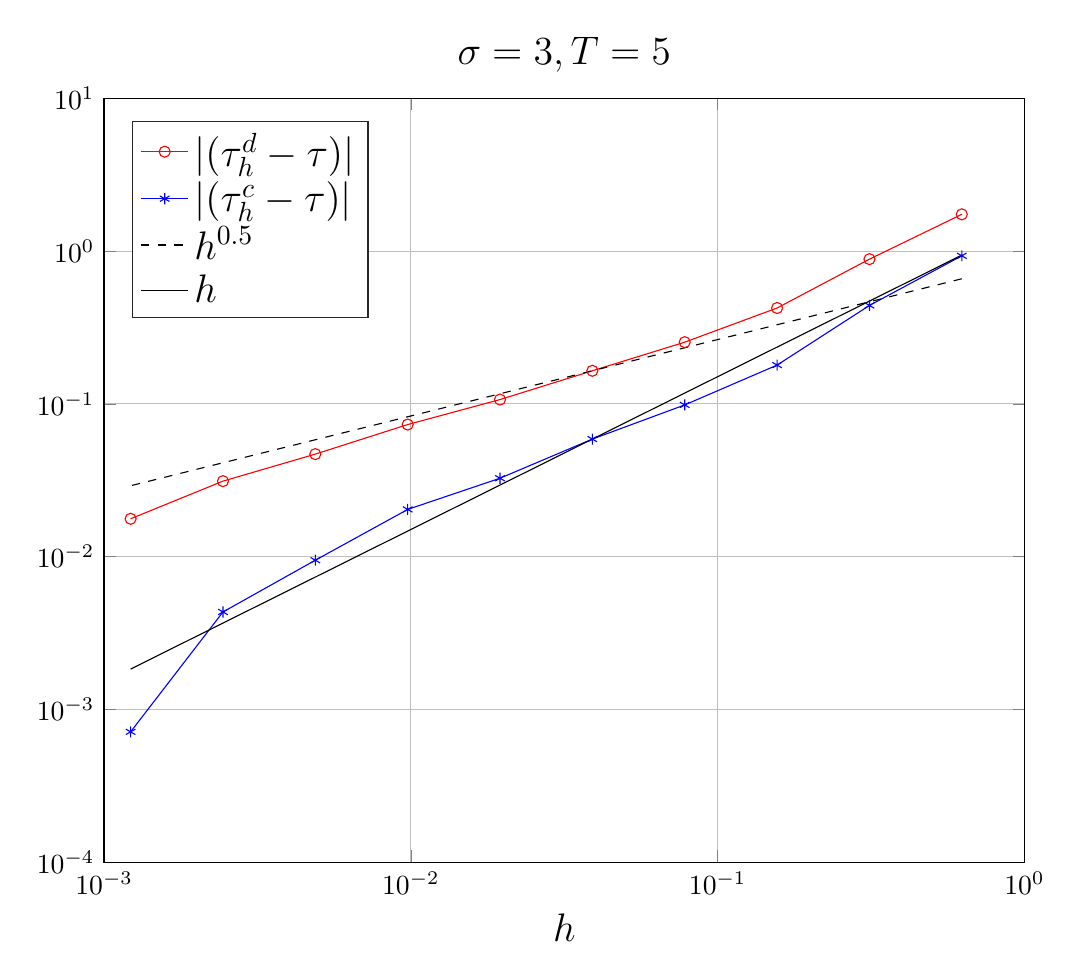
\begin{tikzpicture}

\begin{axis}[%
width=4.602in,
height=3.82in,
at={(0.772in,0.516in)},
scale only axis,
title = {$\sigma = 3, T = 5$},
title style = {font = \Large},
xmode=log,
xmin=0.001,
xmax=1,
xminorticks=false,
xlabel={$h$},
xlabel style={font=\Large},
xmajorgrids,
ymode=log,
ymin=0.0001,
ymax=10,
yminorticks=false,
ymajorgrids,
axis background/.style={fill=white},
legend style={at={(0.03,0.97)},anchor=north west,legend cell align=left,align=left,draw=white!15!black,font=\Large}
]
\addplot [color=red,solid,mark=o,mark options={solid}]
  table[row sep=crcr]{%
0.625	1.73914617431998\\
0.3125	0.885146174319978\\
0.15625	0.423927424319978\\
0.078125	0.253357111819978\\
0.0390625	0.164665705569978\\
0.01953125	0.106693049319978\\
0.009765625	0.0732106274449781\\
0.0048828125	0.0468932446324781\\
0.00244140625	0.0312094067418531\\
0.001220703125	0.0176961010777906\\
};
\addlegendentry{$|\E(\tau_h^d - \tau)|$};

\addplot [color=blue,solid,mark=asterisk,mark options={solid}]
  table[row sep=crcr]{%
0.625	0.931021174319978\\
0.3125	0.440614924319978\\
0.15625	0.179380549319978\\
0.078125	0.098419611819978\\
0.0390625	0.058821955569978\\
0.01953125	0.0326110180699781\\
0.009765625	0.0203737133824781\\
0.0048828125	0.00948064697622808\\
0.00244140625	0.00434612549185309\\
0.001220703125	0.000713688961271941\\
};
\addlegendentry{$|\E(\tau_h^c - \tau)|$};

\addplot [color=black,dashed]
  table[row sep=crcr]{%
0.625	0.658662822279912\\
0.3125	0.465744948149596\\
0.15625	0.329331411139956\\
0.078125	0.232872474074798\\
0.0390625	0.164665705569978\\
0.01953125	0.116436237037399\\
0.009765625	0.082332852784989\\
0.0048828125	0.0582181185186995\\
0.00244140625	0.0411664263924945\\
0.001220703125	0.0291090592593497\\
};
\addlegendentry{$h^{0.5}$};

\addplot [color=black,solid]
  table[row sep=crcr]{%
0.625	0.941151289119649\\
0.3125	0.470575644559824\\
0.15625	0.235287822279912\\
0.078125	0.117643911139956\\
0.0390625	0.058821955569978\\
0.01953125	0.029410977784989\\
0.009765625	0.0147054888924945\\
0.0048828125	0.00735274444624726\\
0.00244140625	0.00367637222312363\\
0.001220703125	0.00183818611156181\\
};
\addlegendentry{$h$};

\end{axis}
\end{tikzpicture}%
 }  
        \caption{Approximation of $\tau$}
        \label{fig:KillOneDPhi}
    \end{subfigure}
    \begin{subfigure}{0.49\linewidth}
        \centering
        \resizebox{1\linewidth}{!}{% This file was created by matlab2tikz.
%
%The latest updates can be retrieved from
%  http://www.mathworks.com/matlabcentral/fileexchange/22022-matlab2tikz-matlab2tikz
%where you can also make suggestions and rate matlab2tikz.
%
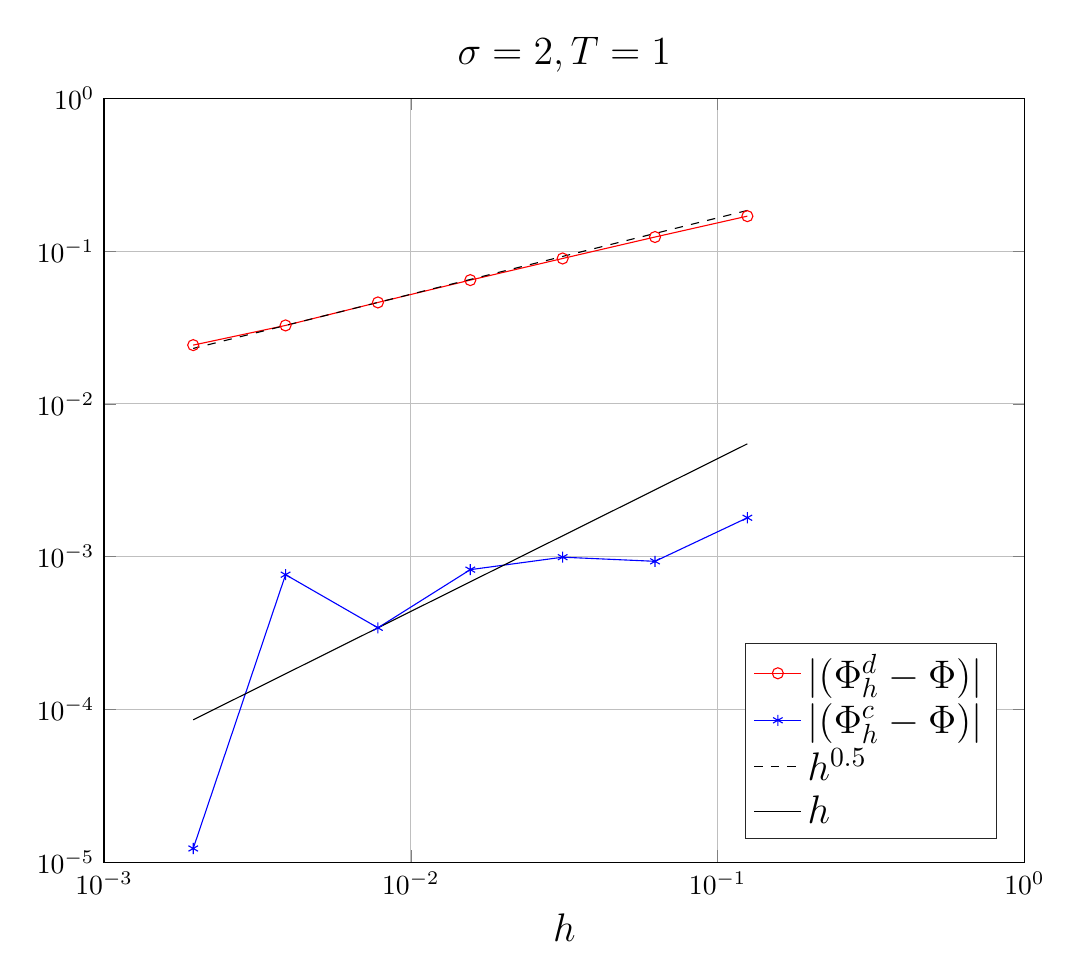
\begin{tikzpicture}

\begin{axis}[%
width=4.602in,
height=3.82in,
at={(0.772in,0.516in)},
scale only axis,
title = {$\sigma = 2, T = 1$},
title style = {font = \Large},
xmode=log,
xmin=0.001,
xmax=1,
xminorticks=false,
xlabel={$h$},
xlabel style = {font=\Large},
xmajorgrids,
ymode=log,
ymin=1e-05,
ymax=1,
yminorticks=false,
ymajorgrids,
axis background/.style={fill=white},
legend pos = south east,
legend style={legend cell align=left,align=left,draw=white!15!black,font=\Large}
]
\addplot [color=red,solid,mark=o,mark options={solid}]
  table[row sep=crcr]{%
0.125	0.169237691826179\\
0.0625	0.123577691826179\\
0.03125	0.0894376918261789\\
0.015625	0.0645576918261789\\
0.0078125	0.0461076918261789\\
0.00390625	0.032607691826179\\
0.001953125	0.024237691826179\\
};
\addlegendentry{$|\E(\Phi_h^d - \Phi)|$};

\addplot [color=blue,solid,mark=asterisk,mark options={solid}]
  table[row sep=crcr]{%
0.125	0.00179769182617895\\
0.0625	0.000932308173821061\\
0.03125	0.000992308173821121\\
0.015625	0.000822308173821118\\
0.0078125	0.000342308173821082\\
0.00390625	0.000762308173821058\\
0.001953125	1.23081738211406e-05\\
};
\addlegendentry{$|\E(\Phi_h^c - \Phi)|$};

\addplot [color=black,dashed]
  table[row sep=crcr]{%
0.125	0.184430767304716\\
0.0625	0.130412246220603\\
0.03125	0.0922153836523578\\
0.015625	0.0652061231103013\\
0.0078125	0.0461076918261789\\
0.00390625	0.0326030615551507\\
0.001953125	0.0230538459130895\\
};
\addlegendentry{$h^{0.5}$};

\addplot [color=black,solid]
  table[row sep=crcr]{%
0.125	0.00547693078113731\\
0.0625	0.00273846539056866\\
0.03125	0.00136923269528433\\
0.015625	0.000684616347642164\\
0.0078125	0.000342308173821082\\
0.00390625	0.000171154086910541\\
0.001953125	8.55770434552705e-05\\
};
\addlegendentry{$h$};

\end{axis}
\end{tikzpicture}%
 }  
        \caption{Approximation of $\Phi$}
        \label{fig:ReflectOneDPhi}
    \end{subfigure}    
    \caption{Results for the one-dimensional case.}
\end{figure}
\end{frame}

\begin{frame}
\frametitle{One-dimensional case - Results}
\begin{figure}[t]
    \centering
    \begin{subfigure}{0.49\linewidth}
        \centering
        \resizebox{1\linewidth}{!}{% This file was created by matlab2tikz.
%
%The latest updates can be retrieved from
%  http://www.mathworks.com/matlabcentral/fileexchange/22022-matlab2tikz-matlab2tikz
%where you can also make suggestions and rate matlab2tikz.
%
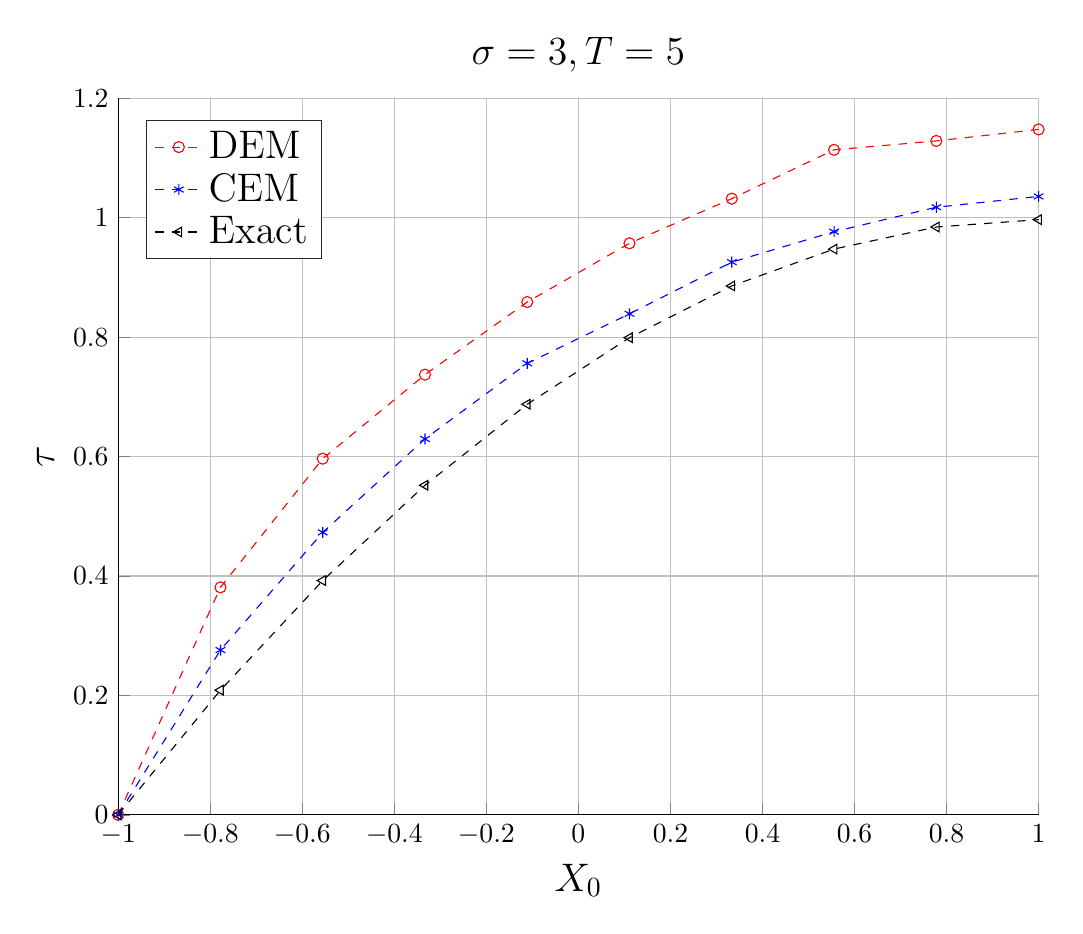
\begin{tikzpicture}

\begin{axis}[%
width=4.602in,
height=3.583in,
at={(0.772in,0.484in)},
scale only axis,
title = {$\sigma = 3, T = 5$},
title style = {font = \Large},
xmin=-1,
xmax=1,
xlabel={$X_0$},
xlabel style={font=\Large},
xmajorgrids,
ymin=0,
ymax=1.2,
ylabel={$\tau$},
ylabel style={font=\Large},
ymajorgrids,
axis background/.style={fill=white},
axis x line*=bottom,
axis y line*=left,
legend pos = north west,
legend style={legend cell align=left,align=left,draw=white!15!black,font=\Large}
]
\addplot [color=red,dashed,mark=o,mark options={solid}]
  table[row sep=crcr]{%
-1	0\\
-0.777777777777778	0.3809765625\\
-0.555555555555556	0.5964609375\\
-0.333333333333333	0.73715625\\
-0.111111111111111	0.8587265625\\
0.111111111111111	0.9571171875\\
0.333333333333333	1.031859375\\
0.555555555555556	1.113609375\\
0.777777777777778	1.1285390625\\
1	1.1478046875\\
};
\addlegendentry{DEM};

\addplot [color=blue,dashed,mark=asterisk,mark options={solid}]
  table[row sep=crcr]{%
-1	0\\
-0.777777777777778	0.275953125\\
-0.555555555555556	0.4729921875\\
-0.333333333333333	0.629484375\\
-0.111111111111111	0.7560703125\\
0.111111111111111	0.8390625\\
0.333333333333333	0.9255703125\\
0.555555555555556	0.976546875\\
0.777777777777778	1.017515625\\
1	1.035609375\\
};
\addlegendentry{CEM};

\addplot [color=black,dashed,mark=triangle,mark options={solid,rotate=90}]
  table[row sep=crcr]{%
-1	0\\
-0.777777777777778	0.208777054487475\\
-0.555555555555556	0.392333503315235\\
-0.333333333333333	0.551939853868488\\
-0.111111111111111	0.687661056545228\\
0.111111111111111	0.79906851214989\\
0.333333333333333	0.885727939207175\\
0.555555555555556	0.947463001823471\\
0.777777777777778	0.984384604394486\\
1	0.996687130893952\\
};
\addlegendentry{Exact};

\end{axis}
\end{tikzpicture}%
 }  
        \caption{Approximation of $\tau$}
        \label{fig:KillOneDPhi}
    \end{subfigure}
    \begin{subfigure}{0.49\linewidth}
        \centering
        \resizebox{1\linewidth}{!}{% This file was created by matlab2tikz.
%
%The latest updates can be retrieved from
%  http://www.mathworks.com/matlabcentral/fileexchange/22022-matlab2tikz-matlab2tikz
%where you can also make suggestions and rate matlab2tikz.
%
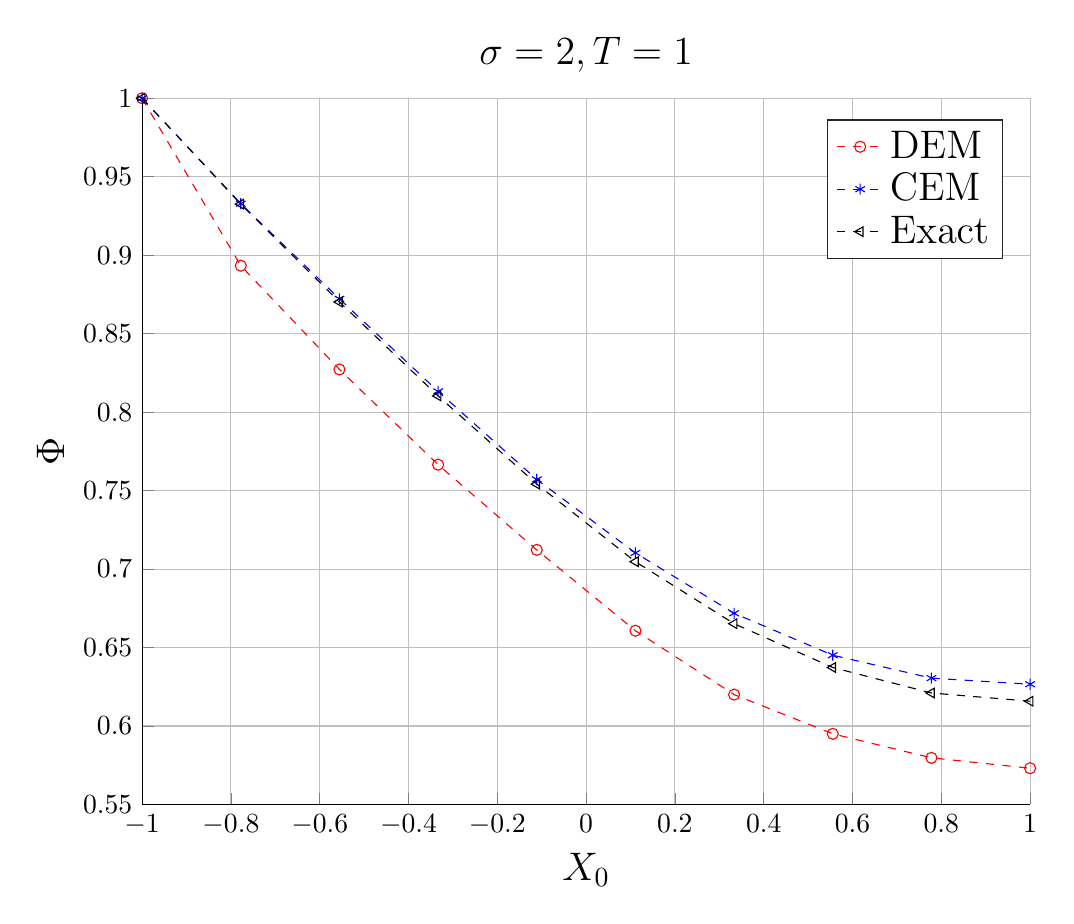
\begin{tikzpicture}

\begin{axis}[%
width=4.44in,
height=3.531in,
at={(0.745in,0.496in)},
scale only axis,
title = {$\sigma = 2, T = 1$},
title style = {font = \Large},
xmin=-1,
xmax=1,
xlabel={$X_0$},
xlabel style={font=\Large},
xmajorgrids,
ymin=0.55,
ymax=1,
ylabel={$\Phi$},
ylabel style={font=\Large},
ymajorgrids,
axis background/.style={fill=white},
axis x line*=bottom,
axis y line*=left,
legend pos = north east,
legend style={legend cell align=left,align=left,draw=white!15!black,font = \Large}
]
\addplot [color=red,dashed,mark=o,mark options={solid}]
  table[row sep=crcr]{%
-1	1\\
-0.777777777777778	0.8933\\
-0.555555555555556	0.8272\\
-0.333333333333333	0.7665\\
-0.111111111111111	0.7122\\
0.111111111111111	0.6607\\
0.333333333333333	0.62\\
0.555555555555556	0.595\\
0.777777777777778	0.5797\\
1	0.5731\\
};
\addlegendentry{DEM};

\addplot [color=blue,dashed,mark=asterisk,mark options={solid}]
  table[row sep=crcr]{%
-1	1\\
-0.777777777777778	0.9328\\
-0.555555555555556	0.8722\\
-0.333333333333333	0.8132\\
-0.111111111111111	0.7571\\
0.111111111111111	0.7103\\
0.333333333333333	0.6718\\
0.555555555555556	0.6451\\
0.777777777777778	0.6305\\
1	0.6266\\
};
\addlegendentry{CEM};

\addplot [color=black,dashed,mark=triangle,mark options={solid,rotate=90}]
  table[row sep=crcr]{%
-1	1\\
-0.777777777777778	0.932548077502788\\
-0.555555555555556	0.870181977112059\\
-0.333333333333333	0.810303153980793\\
-0.111111111111111	0.754108688988762\\
0.111111111111111	0.70469446885863\\
0.333333333333333	0.665180416423286\\
0.555555555555556	0.63727357440893\\
0.777777777777778	0.621019342130665\\
1	0.615785886384429\\
};
\addlegendentry{Exact};

\end{axis}
\end{tikzpicture}%
 }  
        \caption{Approximation of $\Phi$}
        \label{fig:ReflectOneDPhi}
    \end{subfigure}    
    \caption{Approximation of $\tau$ and $\Phi$ with respect to initial value $X_0$.}
\end{figure}
\end{frame}
